In this chapter we provide a general overview of the literature  concerning evolutionary test case generation, in both the Object-Oriented and procedural contexts. 
The main techniques and algorithms employed for the problem will be examined and compared, to act as the base for our study.


\section{EvoSuite}
EvoSuite is an example of an evolutionary algorithm that optimizes the whole test suite towards just one coverage criterion, rather than generating test cases directed towards multiple coverage criteria.
With EvoSuite, any collateral coverage isn't a concern since all coverage is intentional, given that the ultimate goal is to generate the whole test suite.
The algorithm starts with a randomly generated population of test suites.
The fitness function rewards better coverage of the source code; if two suites have the same coverage, the one with fewer statements is chosen. For each test suite, its fitness is measured by executing all of its test cases and keeping track of the executed methods and of the minimal branch distance for each branch.

\begin{itemize}
    \item Expand on bloat in EvoSuite
    \item algorithm pseudocode
\end{itemize}




\newpage
\section{NSGA-II}
A popular algorithm for many-objective search problems is the Non-dominated Sorting Genetic Algorithm II (NSGA-II). This algorithm is based on three principles:

\begin{itemize}
    \item It uses elitism when evolving the population: the most fit individuals are carried over along the offsprings.
    \item It uses an explicit diversity-preserving mechanism, the Crowding distance.
    \item It emphasizes the non-dominated solutions, as its name suggests.
\end{itemize}

In the context of test cases, domination can be expressed by the following relation:
\begin{definition}
    A test case $ x $ dominates another test case $ y $, also written $ x  \prec y $ if and only if ...
\end{definition}

\begin{algorithm}[H]
    \caption{NSGA-II}

    \SetKwInOut{Input}{input}
    \SetKwInOut{Output}{output}
    \SetKwBlock{Beginn}{beginn}{ende}

    \DontPrintSemicolon 
    
    \Input {
        $ U = \{u_1,...,u_m\} $ the set of coverage targets of a program \newline 
        Population size $ M $
    }
    \Output {
        A test suite $ T $ \newline
    }
    \Begin {
        $ t \gets 0 $\;
        $ P_t \gets $ RANDOM-POPULATION($ M $)\;
        
        \While{$ not (search\_budget\_consumed) $}{
            $ Q_t \gets $ GENERATE-OFFSPRING($ P_t $)\;
            $ R_t \gets P_t \cup Q_t $\;
            $ F \gets $ FAST-NONDOMINATED-SORT($ R_t $)\;
            $ P_{t + 1} \gets 0 $\;
            $ d \gets 1 $\;

            \While{$ (|P_{t + 1}| + |F_d| \leqslant M) $}{
                CROWDING-DISTANCE-ASSIGNMENT($ F_d $)
                $ P_{t + 1} \gets P_{t + 1} \cup F_d $\;
                $ d \gets d + 1 $\;
            }

            Sort($ F_d $) // according to the crowding distance\;
            $ P_{t + 1} \gets P_{t + 1} \cup F_d[1: (M - |P_{t + 1}|)] $\;
            $ t \gets t + 1 $\;
        }
        $ S \gets t + 1 $\;
    }
\end{algorithm}

The NSGA-II algorithm works as follows:
\begin{itemize}
    \item Starting from an initial population of individuals Pt, generate an offspring population Qt of equal size and merge the two together, obtaining the population Rt.
    \item Perform non-dominated sorting of the individuals in Rt based on target indicators and classify them by fronts, i.e. they are sorted according to an ascending level of non-domination.  This ensures that the top Pareto-optimal individuals will survive to the next generation.
    \item If one of the fronts in the sorted sequence doesn't fit in terms of population size, crowding distance sorting is performed.
    \item Create the new population based on crowded tournament selection, then perform crossover and mutation. 
\end{itemize}


Figure \ref{fig:NSGA-II algorithm main loop} summarizes the main loop of the algorithm:
\begin{figure}[!h]
    \centering
    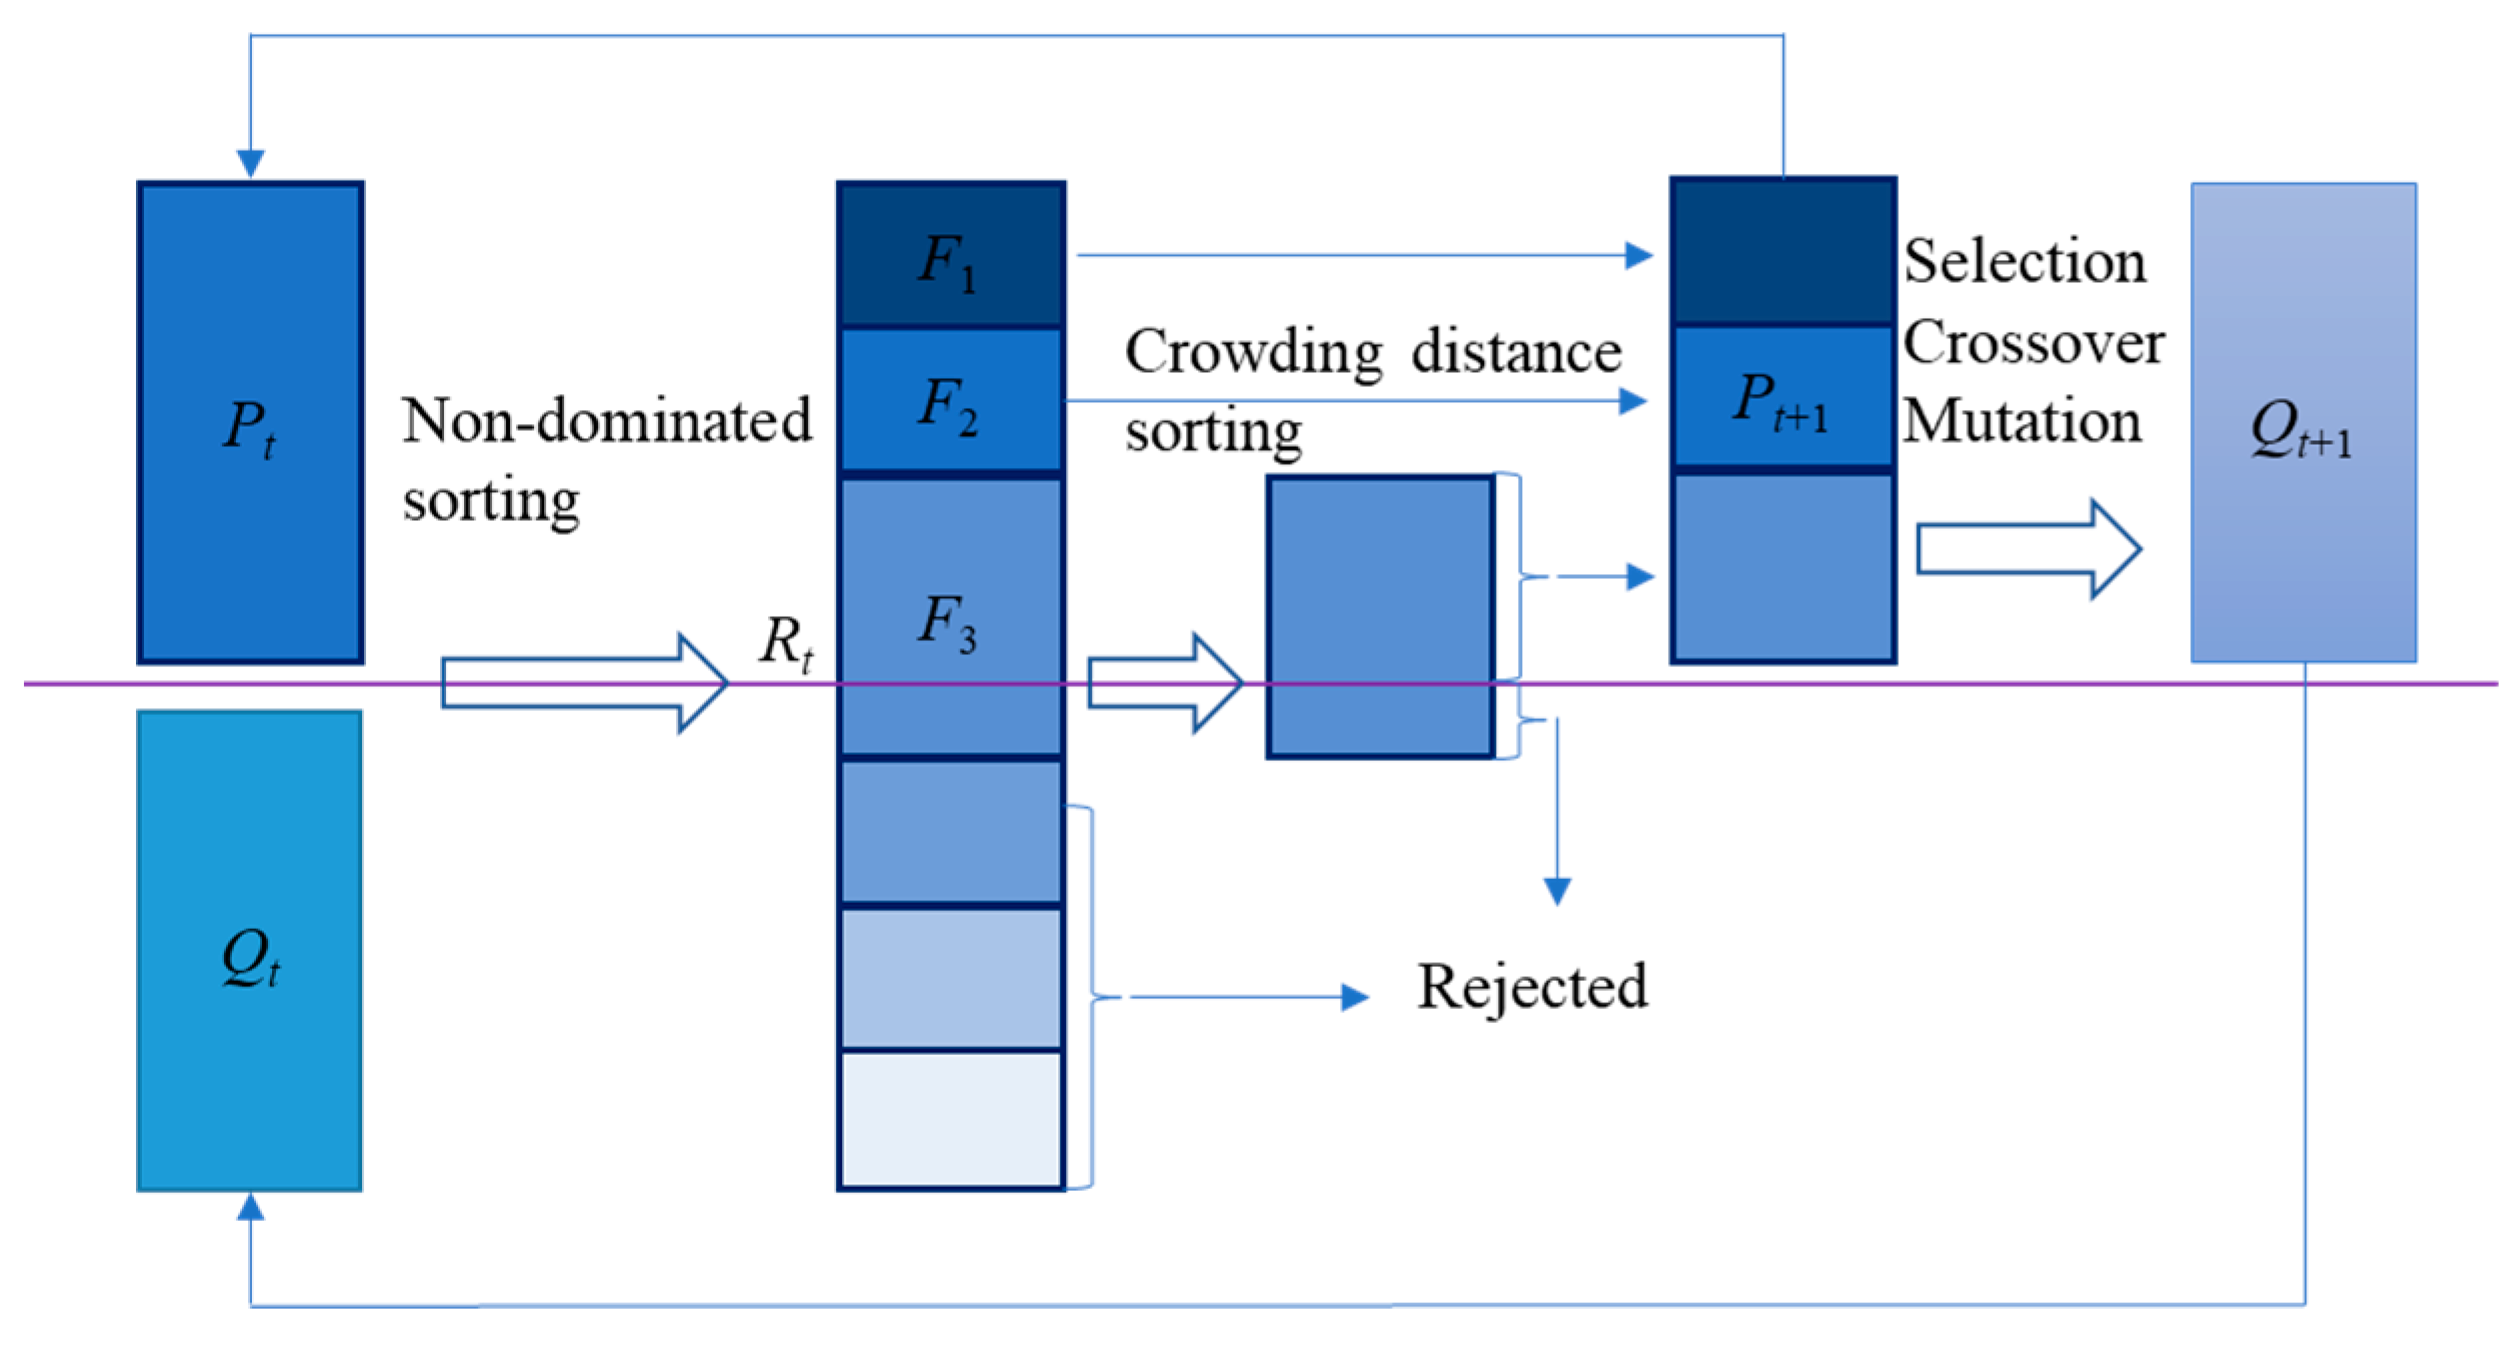
\includegraphics[scale=0.1]{./figures/nsga-ii.png}
    \caption{NSGA-II algorithm main loop.}
    \label{fig:NSGA-II algorithm main loop}
\end{figure}


In the context of software engineering, NSGA-II has been applied to problems such as software refactoring and test case prioritization,
with two or three objectives. If the number of objectives begins to grow, however, the performance of the algorithm doesn't scale up well \cite{DBLP:journals/csur/LiLTY15}.
To overcome these limitations, there have been various adjustments and optimization of this algorithm...





\newpage
\section{SPEA2}
Strength Pareto Evolutionary Algorithm (SPEA) is another multi-objective evolutionary search algorithm based on the concept of Pareto domination for fitness and selection, originally proposed by Zitzler and Thiele in 1999 \cite{DBLP:journals/tec/ZitzlerT99}. SPEA2 was presented as an evolution of the algorithm by the same authors \cite{DBLP:journals/tec/ZitzlerT01}.
A  peculiarity of SPEA2 is that it uses an archive to store non-dominated solutions generated in each iteration; as we will see later, the archive approach is also employed by more modern solutions.
\newline \newline
During the evolution, a strength value is calculated for each individual in each generation and is used for the selection of the fittest individuals. For any solution $ i $, this strength value is measured based on the numbers of $ j $ individuals, belonging to the archive and the population, dominated by $ i $.
\newline 

\begin{algorithm}[H]
    \caption{SPEA2}

    \SetKwInOut{Input}{input}
    \SetKwInOut{Output}{output}
    \SetKwBlock{Beginn}{beginn}{ende}

    \DontPrintSemicolon   

    \Input {
        $ U = \{u_1,...,u_m\} $ the set of coverage targets of a program \newline 
        An archive A \newline
        Population size $ M $
    }
    \Begin {
        $ P_t \gets $ RANDOM-POPULATION($ M $)\;
        \While{$ not (search\_budget\_consumed) $} {
            CALCULATE-STRENGTH($ P_t $, $ A $)\;
            UPDATE-ARCHIVE($ P_t $, $ A $)\;
            BINARY-TOURNAMENT-SELECTION($ P_t $)\;
            CROSOVER($ P_t $)\;
            MUTATION ($ P_t $)\;
        }
    }
\end{algorithm}

If the size of the archive doesn't reach the population size, dominated individuals are used to fill up the remaining spaces.
Similarly to NSGA-II isn't suitable for problems with more than three objectives\cite{DBLP:conf/icccsec/LiuZ19}.





\newpage
\section{MOSA}
The Multi-Objective Sorting Algorithm, MOSA \cite{DBLP:conf/icst/PanichellaKT15} is a GA proposed as an improvement over NSGA-II and SPEA2 for many-objective test case generation, with the main goal of allowing for a higher number of objectives to optimize. With this algorithm, the coverage of the different branches makes up the set of objectives to be optimized. The main characteristic about MOSA is that instead of ranking candidates for selection based on their Pareto optimality, it uses a preference criterion; this criterion selects the test case with the lowest objective score for each uncovered target; these selected individuals are given a higher chance of survival, while other test cases are ranked with the traditional NSGA-II approach.


As the first step, MOSA starts from a randomly generated initial population of test cases. 
To create the next generation, MOSA generates offsprings by implementing the classic operations of selection, crossover and mutation. 
Before selection occurs however, for each uncovered branch, the test case with the lowest objective score(branch distance + approach level) is determined; these test cases will have assigned the rank 0 and will make up the first front. The remainder of the test cases will be sorted according to the traditional NSGA-II approach.

After the rank assignment step is complete, the crowding distance is calculated to determine which individuals to select: the individuals with higher distance from the rest are given a higher chance of being selected. The algorithm attempts to select as many test cases as possible, starting from front 0,  until the population size is reached.



\begin{algorithm}[H]
    \caption{MOSA}

    \SetKwInOut{Input}{input}
    \SetKwInOut{Output}{output}
    \SetKwBlock{Beginn}{beginn}{ende}

    \DontPrintSemicolon   

    \Input {
        $ U = \{u_1,...,u_m\} $ the set of coverage targets of a program \newline 
        Population size $ M $
    }
    \Output {
        A test suite $ T $ \newline
    }
    \Begin {
        $ t \gets 0 $\;
        $ P_t \gets $ RANDOM-POPULATION($ M $)\;
        $ archive \gets $ UPDATE-ARCHIVE($ P_t $, \O)\;

        \While{$ not (search\_budget\_consumed) $}{
            $ Q_t \gets $ GENERATE-OFFSPRING($ P_t $)\;
            $ archive \gets $ UPDATE-ARCHIVE($ Q_t $, $ archive $)\;
            $ R_t \gets P_t \cup Q_t $\;
            $ F \gets $ PREFERENCE-SORTING($ R_t $)\;
            $ P_{t + 1} \gets 0 $\;
            $ d \gets 0 $\;

            \While{$ (|P_{t + 1}| + |F_d| \leqslant M) $}{
                CROWDING-DISTANCE-ASSIGNMENT($ F_d $)
                $ P_{t + 1} \gets P_{t + 1} \cup F_d $\;
                $ d \gets d + 1 $\;
            }

            Sort($ F_d $) // according to the crowding distance\;
            $ P_{t + 1} \gets P_{t + 1} \cup F_d[1: (M - |P_{t + 1}|)] $\;
            $ t \gets t + 1 $\;
        }
        $ T \gets archive $\;
    }
\end{algorithm}


\begin{algorithm}[H]
    \caption{PREFERENCE-SORTING}

    \SetKwInOut{Input}{input}
    \SetKwInOut{Output}{output}
    \SetKwBlock{Beginn}{beginn}{ende}

    \DontPrintSemicolon   

    \Input {
        $ T = \{t_1,...,t_n\} $, a set of candidate test cases \newline 
        Population size $ M $
    }
    \Output {
        A non-dominated ranking assignment $ F $ \newline
    }
    \Begin {
        $ F_0 $ // first front\;
        \For{$ u_i \in U $ and $ u_i $ is uncovered }{
            // for each uncovered test target, the best test case according to the preference criterion is selected\;
            $t_{best} \gets $ test case in T with minimum objective score for $ u_i $\;
            $ F_0 \gets F_0 \cup \{t_{best}\} $\;
        }
        $ T \gets T - F_0 $\;
        \eIf{$ |F_0| > M $}{
            $ F_1 \gets T $\;
        } {
            $ U^* \gets \{u \in U : u $ is uncovered\}\;
            $ E \gets $ FAST-NONDOMINATED-SORT($ T $ , $ \{u \in  U^* \} $)\;
            $ d \gets 0 $\;
            \For{All non-dominated fronts in $ E $}{
                $ F_{d + 1} \gets E_d $\;
            }
        }
    }
\end{algorithm}


\begin{algorithm}[H]
    \caption{DOMINANCE-COMPARATOR}

    \SetKwInOut{Input}{input}
    \SetKwInOut{Output}{output}
    \SetKwBlock{Beginn}{beginn}{ende}

    \DontPrintSemicolon   

    \Input {
        Two test cases to compare, $ t1 $ and $ t2 $\newline 
        $ U = \{u_1,...,u_m\} $ the set of coverage targets of a program
    }
    \Begin {
        $ dominates1 \gets false $\;
        $ dominates2 \gets false $\;
        \For{$ u_i \in U $ and $ u_i $ is uncovered}{
            $ f_i^1 \gets $ values of $ u_i $ for $ t_1 $\;
            $ f_i^2 \gets $ values of $ u_i $ for $ t_2 $\;
            \If{$ f_i^1 < f_i^2 $}{
                $ dominates1 \gets true $\;
            }
            \If{$ f_i^2 < f_i^1 $}{
                $ dominates2 \gets true $\;
            }
            \If{$ dominates1 == true $ and $ dominates2 == true $}{
                break\;
            }
        }
        \eIf{$ dominates1 == dominates2 $}{
                // $ t1 $ and $ t2 $ don't dominate each other\;
        } {
            \eIf{$ dominates1 == true $} {
                // $ t1 $ dominates $ t2 $\;
            } {
                // $ t2 $ dominates $ t1 $\;
            }
        }
    }
\end{algorithm}

\newpage
Finally, MOSA uses an archived population that keeps track of the best performing test cases, in order to form the final test suite. The archive is continuously updated as follows:

\begin{algorithm}[H]
    \caption{UPDATE-ARCHIVE}

    \SetKwInOut{Input}{input}
    \SetKwInOut{Output}{output}
    \SetKwBlock{Beginn}{beginn}{ende}

    \DontPrintSemicolon   

    \Input {
        A set of candidate test cases $ T $\newline 
        An archive $ A $
    }
    \Output {
        An updated archive $ A $ \newline
    }
    \Begin {
        \For{$ u_i \in U $}{
            $ t_{best} \gets $ \O \;
            $ best_length \gets \infty $\;
            \If{$ u_i $ already covered}{
                $ t_{best} \gets $ test case in $ A $ covering $ u_i $\;
                $ best_length \gets $ number of statements in $ t_best $\;
            }
            \For{$ t_j \in T $}{
                $ score \gets $ objective score of $ t_j $ for target $ u_i $\;
                $ length \gets $ number of statements in $ t_j $\;
                \If{$ score == 0 $ and $ length \leq best_length $}{
                    replace $ t_best $ with $ t_j $ in $ A $\;
                    $ t_best \gets t_j $\;
                    $ best_length \gets length $\;
                }
            }
        }
        return $ A $\;
    }
\end{algorithm}





\newpage
\section{DynaMOSA}
One of the limitations of MOSA is its inability to consider the implicit dependencies between targets, which simply appear as independent objectives to optimize. Such dependencies can be quite common in practice: most commonly, there exist branches which may only be satisfied if and only if other branches in the outer scope have been already covered. 
\\\\
DynaMOSA, Dynamic Many-Objective Sorting Algorithm \cite{DBLP:journals/tse/PanichellaKT18} is an algorithm that focuses on these dynamic dependencies, and has been proposed as an evolution of MOSA. 
Before introducing the algorithm, a few definitions are needed \cite{DBLP:journals/tse/PanichellaKT18}:

\begin{definition}
    (Dominator): A statement $ s1 $ dominates another statement $ s2 $ if every execution path to $ s2 $ passes through $ s1 $.
\end{definition}
\begin{definition}
    (Post-dominator): A statement $ s1 $ post-dominates another statement $ s2 $ if every execution path from $ s2 $ to the exit point passes through $ s1 $. 
\end{definition}
\begin{definition}
    (Control dependency): There is a control dependency between program statement $ s1 $ and program statement $ s2 $ iff: $ (1) s2 $ is not a postdominator of $ s1 $, and $ (2) $ there exist a path in the control flow graph between $ s1 $ and $ s2 $ whose nodes are postdominated by $ s2 $.
\end{definition}
\begin{definition}
    (Control dependency graph): The graph $ G = \langle N, E, s \rangle $, consisting of nodes $ n \in N $ that represent program statements, and edges $ e \in E \subseteq N X N $ that represent control dependencies between program statements, is called control dependency graph. Node $ s \in N $ represents the entry node, which is connected to all nodes that are not under the control dependency of another node.
\end{definition}


This definition can be extended to other coverage criteria. For example, given two branches $ b1 $ and $ b2 $,  we say that $ b1 $ holds a control dependency on $ b2 $ if $ b1 $ is postdominated by a statement $ s1 $ which holds a control dependency on a node $ s2 $ that postdominates $ b2 $.

DynaMOSA uses the control dependency graph to identify which targets are independent from each other and which ones can be covered only after satisfying previous targets in the graph.
Algorithm 6 highlights the test case evolution in DynaMOSA.

\begin{algorithm}[H]
    \caption{DynaMOSA}

    \SetKwInOut{Input}{input}
    \SetKwInOut{Output}{output}
    \SetKwBlock{Beginn}{beginn}{ende}

    \DontPrintSemicolon   

    \Input {
        $ U = \{u_1,...,u_m\} $ the set of coverage targets of a program \newline 
        Population size $ M $ \newline
        $ G = \langle N, E, s \rangle $: control dependency graph of the program \newline
        $ \phi: E \rightarrow U: $ partial mapping between edges and targets
    }
    \Output {
        A test suite $ T $ \newline
    }
    \Begin {
        $ U^* \gets $ targets in $ U $ with not control dependencies\;
        $ t \gets 0 $\;
        $ P_t \gets $ RANDOM-POPULATION($ M $)\;
        $ archive \gets $ UPDATE-ARCHIVE($ P_t $, \O)\;
        $ U^* \gets $ UPDATE-TARGETS($ U^* $, $ G $, $ \phi $)\;

        \While{$ not (search\_budget\_consumed) $}{
            $ Q_t \gets $ GENERATE-OFFSPRING($ P_t $)\;
            $ archive \gets $ UPDATE-ARCHIVE($ Q_t $, $ archive $)\;
            $ U^* \gets $ UPDATE-TARGETS($ U^* $, $ G $, $ \phi $)\;
            $ R_t \gets P_t \cup Q_t $\;
            $ F \gets $ PREFERENCE-SORTING($ R_t $, $ U^* $)\;
            $ P_{t + 1} \gets 0 $\;
            $ d \gets 0 $\;

            \While{$ (|P_{t + 1}| + |F_d| \leqslant M) $}{
                CROWDING-DISTANCE-ASSIGNMENT($ F_d $, $ U^* $)
                $ P_{t + 1} \gets P_{t + 1} \cup F_d $\;
                $ d \gets d + 1 $\;
            }

            Sort($ F_d $) // according to the crowding distance\;
            $ P_{t + 1} \gets P_{t + 1} \cup F_d[1: (M - |P_{t + 1}|)] $\;
            $ t \gets t + 1 $\;
        }
        $ T \gets archive $\;
    }
\end{algorithm}


\newpage
The main difference with MOSA is how the initial target population is selected; with DynaMOSA, only the targets that are free from dependencies are part of this set.
Then, in each iteration, the set of non-dependent targets is updated by using the following procedure:
\\

\begin{algorithm}[H]
    \caption{UPDATE-TARGETS}

    \SetKwInOut{Input}{input}
    \SetKwInOut{Output}{output}
    \SetKwBlock{Beginn}{beginn}{ende}
    \SetKwProg{Fn}{function}{:}{}

    \DontPrintSemicolon   

    \Input {
        $ G = \langle N, E, s \rangle $: control dependency graph of the program \newline
        $ U^*  \subseteq U $: current set of targets \newline 
        $ \phi: E \rightarrow U: $ partial mapping between edges and targets
    }
    \Output {
        $ U^* $: updated set of targets to optimize
    }
    \Begin {
        \For{$ u \in U $}{
            \If{$ u $ is covered}{
                $ U^* \gets U^* - \{u\} $\;
                $ e_u \gets $ edge in $ G $ for the target $ u $\;
                visit($ e_u $)\;
            }
        }
    }
    
    \Fn{visit($ e_u \in E $)} {
        \For{each unvisited $e_n \in E $ control depenmdent on $ e_u $}{
            \eIf{$ \phi(e_n) $ is not covered} {
                $ U^* \gets U^* \cup \{\phi(e_n)\} $\;
                set $ e_n $ as visited\;
            } {
                visit($ e_m $)\;
            }
        }
    }
\end{algorithm}

This routine update the sets of selected targets $ U^* $ in order to include any uncovered targets that are control dependent on the newly covered target.
In the case of newly covered targets, the procedure iterates over the control graph to find all control dependent targets.





\newpage
\section{OCELOT and object-oriented versus procedural test case generation}
Generally speaking, both EvoSuite and MOSA/DynaMOSA have been designed with the OO paradigm in mind, as well as most empirical software engineering tools for testing.

\textbf{...expand on automated testing for procedural programs...}

Optimal Coverage sEarch-based tooL for sOftware Testing, OCELOT \cite{DBLP:conf/ssbse/ScalabrinoGNOL16} is a test case generation tool for C programs that implements both a multi-objective approach based on MOSA, and a new iterative single-target approach named LIPS, Linear Independent Path-based Search.
OCELOT can automatically detect the input types of a C function, without requiring any specification of parameters; Additionally it can handle the different data types of C, including pointers and structs, and produces test cases based on the Check framework \cite{Check}.
Similarly to other tools, OCELOT is not able to generate oracles.
From an implementation point of view, the GA implementation in OCELOT was realized with the JMetal, a Java framework for multi-objective optimization with meta-heuristics \cite{JMetal}. Furthermore, JNI is used as interface with the target program to try different combinations of test data.
SBX Crossover, Polynomial Mutation and Binary Tournament Selection, for both the multi-objective and iterative approaches.

The iterative approach used in OCELOT, LIPS

Running OCELOT consists of two main phases: build and run \cite{DBLP:conf/kbse/ScalabrinoGNGLG18}, as highlighted in figure \ref{fig:OCELOT main loop}:

\begin{figure}[!h]
    \centering
    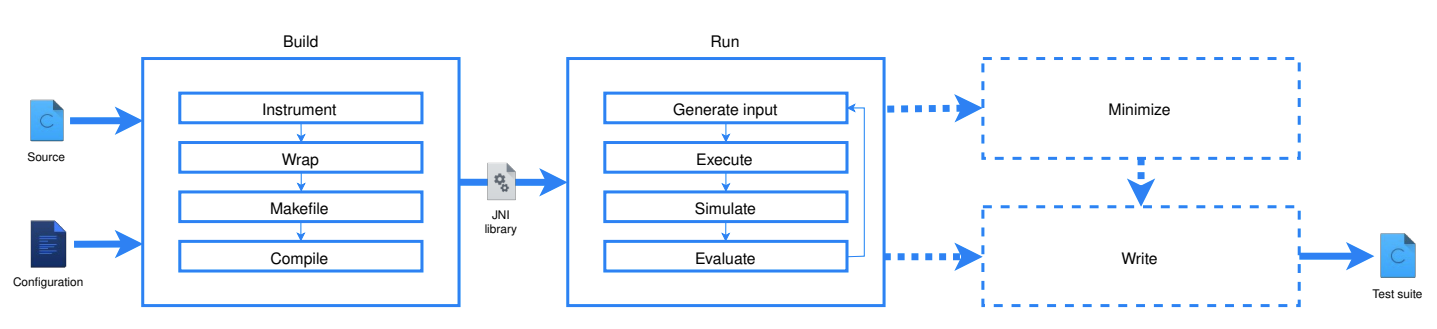
\includegraphics[scale=0.35]{figures/OCELOT_workflow.PNG}
    \caption{OCELOT components and workflow.}
    \label{fig:OCELOT main loop}
\end{figure}





\newpage
\section{Test case generation for CyberPhysical Systems}
Typically, in the development stages of a CPS, validation and verification happen according to the V-model approach.

AmbieGen based on NSGA-II.
Markov chains used to assign values to different attributes


\cite{DBLP:journals/infsof/HumeniukKA22}
\cite{CPS:Model-based}